\documentclass[11pt]{article}
\usepackage[T1]{fontenc}
\usepackage[utf8]{inputenc}
\usepackage{lmodern}
\usepackage[margin=1in]{geometry}
\usepackage{microtype}
\usepackage{amsmath,amssymb}
\usepackage{booktabs}
\usepackage{tabularx}
\usepackage{array}
\usepackage{multirow}
\usepackage{enumitem}
\usepackage[font=small,labelfont=bf]{caption}
\usepackage{float}
\usepackage{xcolor}
\usepackage{tikz}
\usetikzlibrary{positioning,arrows.meta,calc,fit,shapes.geometric}
\usepackage[numbers,sort&compress]{natbib}
\usepackage[hidelinks]{hyperref}
\usepackage{url}

\newcommand{\aosi}{AOSI}
\newcommand{\Lay}[1]{L#1}
% Coverage marks for the comparison table
\DeclareRobustCommand{\full}{\tikz[baseline=-0.6ex]\fill (0,0) circle (2.3pt);}
\DeclareRobustCommand{\half}{\tikz[baseline=-0.6ex]{\draw (0,0) circle (2.3pt);\fill (0,0) -- (90:2.3pt) arc (90:270:2.3pt) -- cycle;}}
\DeclareRobustCommand{\none}{\tikz[baseline=-0.6ex]\draw (0,0) circle (2.3pt);}
\newcolumntype{Y}{>{\raggedright\arraybackslash}X}
\newcolumntype{C}{>{\centering\arraybackslash}p{0.95cm}}

\setlength{\textfloatsep}{10pt plus 2pt minus 2pt}
\setlength{\floatsep}{8pt plus 2pt minus 2pt}
\setlength{\intextsep}{8pt plus 2pt minus 2pt}
\definecolor{l7}{HTML}{3B4A6B}
\definecolor{l6}{HTML}{2F6DB5}
\definecolor{l5}{HTML}{2E9C8F}
\definecolor{l4}{HTML}{4E9F3D}
\definecolor{l3}{HTML}{E0A126}
\definecolor{l2}{HTML}{D9692B}
\definecolor{l1}{HTML}{C0392B}

\title{The AI Open Systems Interconnection (AOSI) Reference Model:\\
A Seven-Layer Vocabulary for Locating Performance, Correctness\\
and Security Concerns in Generative AI Inference}
\author{Divyendu Bhatt\\
\small Independent Researcher\\
\small \texttt{Divyendu.bhatt@gmail.com}}
\date{9 November 2026}

\begin{document}
\maketitle

\begin{abstract}
A single generative AI request crosses a client application, an orchestration gateway, a retrieval pipeline, an inference-serving engine, a transformer model, a compiler and runtime stack, and accelerator hardware. Each tier has its own tools, telemetry and vocabulary, and practitioners lack a shared frame for stating \emph{where} in this path a latency regression, a quality failure or a security threat originates. Standards, risk frameworks, industry stack diagrams, serving surveys and threat catalogues each cover part of this problem, and existing OSI-inspired AI models target agent cognition or multi-agent interoperability rather than the execution path of one request. This paper presents AOSI, an informative seven-layer reference model for generative AI inference that (i) orders the tiers from physical infrastructure (L1) to application (L7), (ii) names a canonical data state at every layer boundary, from JSON payload to silicon voltages, (iii) derives a layer-isolation method for diagnosing latency and failures, and (iv) maps the OWASP Top 10 for LLM Applications onto the layers at which each risk materialises. We position AOSI against eleven groups of related work in a structured comparison, illustrate its use on a worked (non-empirical) triage example, and state its limitations: it has not been empirically validated or adopted by any standards body. We close with a concrete evaluation plan.
\end{abstract}

\noindent\textbf{Keywords:} reference model, generative AI, LLM inference serving, observability, AI security, layered architecture

\section{Introduction}
\label{sec:intro}

Production generative AI is no longer a model behind an API. Serving a single chat completion with retrieval-augmented generation (RAG)~\cite{lewis2020rag} involves an application client, an API or AI gateway that applies policy and templates, an embedding model and vector index, a serving engine that batches requests and manages a key--value (KV) cache~\cite{yu2022orca,kwon2023paged}, the transformer itself, a framework and compiler stack that lowers the model to kernels~\cite{dao2022flash}, and accelerators whose memory bandwidth often bounds decode speed~\cite{williams2009roofline,yuan2024roofline}. These tiers are usually owned by different teams, observed with different tools, and described with different words.

The consequence is a recurring practical problem: \emph{there is no shared vocabulary for locating a failure or threat along the generative AI execution path}. A report that ``the model is slow'' may mean retrieval latency, queueing in the serving engine, KV-cache preemption, or memory-bandwidth saturation on the device; ``the model hallucinated'' may mean a retrieval miss, a stale index, a prompt-template defect, or a quantisation regression. Security controls are often specified as generic ``AI controls'' without stating the tier at which the threat materialises. Sculley et al.\ observed that ML systems erode abstraction boundaries and accumulate system-level debt~\cite{sculley2015debt}; generative inference stacks inherit that problem with more tiers.

Computer networking faced an analogous problem and addressed it with the OSI Basic Reference Model~\cite{iso7498,itux200,zimmermann1980osi}: a fixed set of layers, service boundaries between adjacent layers, and named data units at each boundary. OSI's lasting value has arguably been less its protocols than its vocabulary: engineers can say ``this is a layer-2 problem'' and be understood.

This paper applies the same \emph{method}---not the OSI layers themselves---to generative AI inference. We are not the first to draw an OSI analogy for AI (Section~\ref{sec:related}); our contribution is narrower and, we argue, complementary. Specifically:

\begin{enumerate}[leftmargin=*,itemsep=2pt]
  \item \textbf{A full-depth, ordered layer model of single-request generative inference} (Section~\ref{sec:model}), spanning application (L7), orchestration and gateway (L6), retrieval and knowledge (L5), inference and serving (L4), model and weight architecture (L3), framework and runtime (L2), and physical infrastructure (L1), with explicit scope boundaries and design principles.
  \item \textbf{A named data state at every boundary}: JSON payload $\rightarrow$ enriched prompt $\rightarrow$ vector chunks $\rightarrow$ batched tensors $\rightarrow$ hidden states $\rightarrow$ tensor IR $\rightarrow$ silicon voltages, playing the role of OSI protocol data units.
  \item \textbf{A layer-isolation diagnostic method} (Section~\ref{sec:diag}) that combines a latency decomposition, per-layer trace attribution and single-variable isolation tests, including discriminators for three commonly confused causes (L5 retrieval lag, L4 KV-cache pressure, L1 memory-bandwidth saturation).
  \item \textbf{A layer-indexed security mapping} (Section~\ref{sec:security}) that places each OWASP Top 10 for LLM Applications (2025) risk~\cite{owasp2025llm} at the layer(s) where it materialises.
  \item \textbf{A structured comparison} (Section~\ref{sec:related}, Table~\ref{tab:compare}) with eleven groups of related standards, frameworks and layer models, and an \textbf{evaluation plan} (Section~\ref{sec:discussion}) for testing the model's claims.
\end{enumerate}

AOSI is a conceptual, informative model. It defines no protocol, it has not been empirically validated, and it has not been adopted by any standards development organisation. A full specification, including per-layer interfaces, metrics, failure modes and proposed telemetry attributes, is archived as a versioned technical report~\cite{bhatt2026zenodo}; an IETF Internet-Draft version has been prepared for submission to the Independent Submission stream.

\section{Background: Why Layered Reference Models Work}
\label{sec:background}

Layering as a structuring discipline predates networking. Dijkstra's THE system organised an operating system into levels, each relying only on services of the levels below~\cite{dijkstra1968the}, and Parnas argued that modules should be chosen to hide design decisions likely to change~\cite{parnas1972criteria}. The OSI model turned these ideas into a \emph{reference} model for an industry~\cite{zimmermann1980osi,iso7498}. Three properties are relevant here.

\paragraph{Separation of concerns with stable boundaries.} Each OSI layer provides a service to the layer above through a defined boundary. Implementations of one layer can change without changing its neighbours, provided the service is preserved.

\paragraph{Named data units.} OSI names what crosses each boundary (frames, packets, segments, and so on). A named unit can be captured, decoded and measured, which is what makes tools such as protocol analysers effective: an engineer can inspect the unit at a boundary and assert which layer misbehaved.

\paragraph{Reference, not implementation.} ISO/IEC 7498-1 explicitly positions the model as a framework for coordinating standards, not an implementation specification~\cite{iso7498}. The Internet's own protocols do not map one-to-one onto OSI layers, yet the vocabulary remained useful. The end-to-end argument~\cite{saltzer1984e2e} adds a caution that transfers directly to AI: some functions (e.g., correctness of the final answer) can only be fully implemented with knowledge held at the endpoints, so a layer model must not pretend that every concern is local to one layer.

Distributed tracing supplies the other ingredient AOSI relies on. Dapper showed that propagating a trace context across service boundaries makes latency in large distributed systems attributable to individual components~\cite{sigelman2010dapper}; W3C Trace Context and the OpenTelemetry generative AI semantic conventions standardise parts of this for modern stacks~\cite{w3ctracecontext,otelgenai}. AOSI's diagnostic method (Section~\ref{sec:diag}) is essentially a proposal for \emph{which} boundaries such traces should mark in a generative AI system.

\section{Related Work}
\label{sec:related}

We group related work into five families and summarise the comparison in Table~\ref{tab:compare}. The assessments are the author's reading of each work's public text or official description; ISO/IEC standards were assessed from their published scope statements, since full texts are not freely available. Corrections are welcome.

\paragraph{International standards and risk frameworks.} ISO/IEC 22989 establishes AI concepts and terminology~\cite{iso22989}. ISO/IEC 23053 provides a technology-neutral framework describing the components and functions of AI systems that use machine learning~\cite{iso23053}. Both are normative and broad: they define \emph{what} an AI system consists of, across the ML lifecycle, rather than how one inference request traverses a serving stack. The NIST AI Risk Management Framework~\cite{nist2023airmf} and its Generative AI Profile~\cite{nist2024genai} define organisational risk-management functions (Govern, Map, Measure, Manage) and generative-AI-specific risks and actions; they are process frameworks rather than technical layer models. AOSI is intended to sit beneath these: it offers a technical location (e.g., ``L5'') at which a ``Measure'' or ``Manage'' activity can be scoped, and it defers to ISO/IEC 22989 for general AI terms.

\paragraph{Industry stack diagrams and MLOps architectures.} The a16z reference architecture for LLM applications~\cite{a16z2023llm} describes data pipelines, embedding models, vector databases, orchestration, APIs and plugins, LLM caches, logging and validation, and app hosting. It is widely referenced and covers roughly AOSI L5--L7, but it treats the model as a hosted API and does not decompose serving, model, framework or hardware tiers. MLOps references---Google Cloud's continuous-delivery architecture~\cite{googlemlops} and Kreuzberger et al.'s literature- and interview-based definition of MLOps components, roles and workflows~\cite{kreuzberger2022mlops}---are organised around the ML \emph{lifecycle} (training, validation, deployment, monitoring). They include model serving and monitoring components but not the internal layering of a generative inference request. AOSI excludes training (Section~\ref{sec:scope}), which is precisely where lifecycle models apply.

\paragraph{Software-architecture research on foundation-model systems.} Lu et al.\ propose a taxonomy of foundation-model-based systems~\cite{lu2023taxonomy}, a pattern-oriented reference architecture for responsible FM-based systems organised into system, operation and supply-chain layers~\cite{lu2023rafm}, and a reference architecture for FM-based agents~\cite{lu2024agents}. These works treat RAG, guardrails and responsible-AI controls as architectural elements and evaluate completeness by mapping to real systems. Their unit of analysis is the software architecture and its design decisions; AOSI's unit is the execution path of a request down to hardware, with named boundary states. The two are complementary: a Lu et al.\ guardrail pattern would be located at AOSI L6, a RAG pattern at L5.

\paragraph{Serving-systems research and surveys.} Systems work such as Orca's iteration-level scheduling~\cite{yu2022orca}, PagedAttention~\cite{kwon2023paged}, chunked prefill~\cite{agrawal2023sarathi} and prefill/decode disaggregation~\cite{zhong2024distserve} shows that the serving tier has its own bottlenecks, distinct from model architecture and hardware. Surveys organise this space: Miao et al.\ span algorithmic and system techniques~\cite{miao2023serving}; Li et al.\ group recent advances into KV-cache and memory management, computation optimisation, cloud deployment and emerging areas including RAG and mixture-of-experts~\cite{li2024servingsurvey}; Pan and Li structure inference systems from request-processing operators to memory management and multi-replica designs~\cite{pan2025inference}; Yuan et al.\ use the roofline model~\cite{williams2009roofline} to explain why decoding is often memory-bound~\cite{yuan2024roofline}. MLPerf Inference provides system-level benchmarks~\cite{reddi2019mlperf}. These works are taxonomies of \emph{optimisation techniques} or measurements, not reference models with layer boundaries and boundary states; AOSI draws on them as evidence that L4, L3, L2 and L1 deserve separate layers.

\paragraph{OSI-inspired AI layer models.} At least two prior works use the OSI analogy explicitly. The ACE framework of Shapiro et al.\ is a six-layer cognitive architecture for autonomous agents, from an Aspirational Layer to Task Prosecution, explicitly inspired by OSI~\cite{shapiro2023ace}. Rodrigo-Gin\'es proposes a seven-level OSI-inspired interoperability stack for agentic AI, from physical infrastructure and runtime execution to agent-to-agent communication, coordination workflows, and governance and trust~\cite{rodrigogines2025osi}. ACE layers an agent's reasoning and control; Rodrigo-Gin\'es layers interoperability between agents. Neither decomposes the inference path within a single request or defines boundary data states for it. AOSI's reserved Layer~8 (agentic workflows; Section~\ref{sec:discussion}) is where these models would connect.

\paragraph{AI security catalogues.} The OWASP Top 10 for LLM Applications (2025)~\cite{owasp2025llm} ranks risk categories; MITRE ATLAS catalogues adversary tactics and techniques against AI-enabled systems~\cite{mitreatlas}; NIST AI 100-2 E2025 provides a taxonomy and terminology of adversarial ML attacks and mitigations~\cite{nist2025aml}; Google's SAIF frames security practices for AI systems~\cite{googlesaif}. These describe \emph{what} can go wrong and what to do; none of them is organised by the execution layer at which a threat materialises. Section~\ref{sec:security} uses AOSI as such an index.

\begin{table}[!htbp]
\centering
\caption{Comparison of AOSI with related standards, frameworks and layer models. \full~= explicit, distinct element; \half~= discussed but not as a distinct layer or boundary; \none~= not a focus. ``States'' = a named data representation at each inter-layer boundary. ``Diag.'' = a method for attributing latency or failures to a tier; ``Sec.'' = security threats or controls addressed (layer-indexed only in AOSI); ``HW'' = hardware layer; ``Serve'' = inference-serving layer. Assessments reflect the author's reading of public descriptions (Section~\ref{sec:related}).}
\label{tab:compare}
\footnotesize
\setlength{\tabcolsep}{2pt}
\begin{tabularx}{\textwidth}{@{}>{\raggedright\arraybackslash}p{2.75cm}YCCCCCC>{\raggedright\arraybackslash}p{1.95cm}@{}}
\toprule
\textbf{Work} & \textbf{Primary scope} & \textbf{HW} & \textbf{Serve} & \textbf{RAG} & \textbf{States} & \textbf{Diag.} & \textbf{Sec.} & \textbf{Nature}\\
\midrule
ISO/IEC 22989~\cite{iso22989} & AI concepts \& terminology & \none & \none & \none & \none & \none & \half & Normative std.\\
ISO/IEC 23053~\cite{iso23053} & ML system components \& functions & \none & \half & \none & \none & \none & \none & Normative std.\\
NIST AI RMF / 600-1~\cite{nist2023airmf,nist2024genai} & Organisational AI risk process & \none & \none & \none & \none & \none & \half & Voluntary guidance\\
a16z LLM app stack~\cite{a16z2023llm} & LLM application tier (\(\approx\)L5--L7) & \none & \half & \full & \none & \none & \half & Industry, inform.\\
MLOps refs.~\cite{googlemlops,kreuzberger2022mlops} & ML lifecycle (CI/CD/CT) & \half & \half & \none & \none & \half & \none & Industry / academic\\
Lu et al.~\cite{lu2023rafm,lu2024agents} & FM-based system \& agent design patterns & \none & \half & \full & \none & \none & \half & Academic, inform.\\
Serving surveys~\cite{miao2023serving,li2024servingsurvey,pan2025inference} & Serving optimisation techniques & \half & \full & \half & \none & \none & \none & Academic surveys\\
ACE~\cite{shapiro2023ace} & Agent cognition, 6 layers & \none & \none & \none & \none & \half & \none & Academic, inform.\\
Rodrigo-Gin\'es~\cite{rodrigogines2025osi} & Multi-agent interoperability, 7 levels & \full & \half & \none & \none & \none & \half & Position paper\\
OWASP LLM Top 10~\cite{owasp2025llm} & LLM application risk list & \none & \half & \full & \none & \none & \full & Community, inform.\\
MITRE ATLAS~\cite{mitreatlas} & Adversary TTP knowledge base & \none & \half & \half & \none & \none & \full & Community, inform.\\
\midrule
\textbf{AOSI (this work)} & \textbf{Single-request GenAI inference, L1--L7} & \full & \full & \full & \full & \full$^{a}$ & \full$^{a}$ & \textbf{Informative proposal}\\
\bottomrule
\end{tabularx}
\par\smallskip\raggedright\footnotesize $^{a}$Proposed method and mapping; not yet empirically validated (Section~\ref{sec:discussion}).
\end{table}

\paragraph{Positioning.} Table~\ref{tab:compare} shows the gap AOSI targets. Works that reach the hardware either layer agents (Rodrigo-Gin\'es) or catalogue optimisations (serving surveys); works that cover RAG and guardrails stop at the model API; security catalogues are not layer-indexed; and none defines a named data state at every boundary. AOSI's claim is therefore \emph{not} that it is the first layered or OSI-style model for AI, but that it combines (a) full-depth coverage of one request's execution path, (b) named boundary states, (c) a diagnostic method built on them and (d) a layer-indexed security mapping. Whether this combination is useful is an empirical question we have not yet answered (Section~\ref{sec:eval}).

\section{The AOSI Model}
\label{sec:model}

\subsection{Scope}
\label{sec:scope}
AOSI covers \emph{inference-time} execution of generative models---primarily autoregressive transformer language models and, by extension, multimodal models---from client request to device execution and back. Training and fine-tuning pipelines, data governance upstream of the retrieval index, wire protocols, API schemas and certification are out of scope. Named products are illustrative occupants of a layer, not endorsements.

\subsection{Design principles}
AOSI's layer definitions are governed by seven principles: (P1) single primary responsibility per layer, with cross-layer components described once per layer they occupy; (P2) a named data state at every boundary; (P3) adjacency of interfaces, with any cross-layer shortcut documented as an explicit coupling; (P4) observability by construction, with telemetry emitted at boundaries and attributable to one layer; (P5) technology neutrality; (P6) awareness of a cost gradient---latency and computational cost increase toward lower layers, while semantic abstraction and policy surface increase toward upper layers; and (P7) security controls placed at the layer where a threat materialises, with defence-in-depth at adjacent layers where justified.

\subsection{Layers}

\begin{figure}[!htbp]
\centering
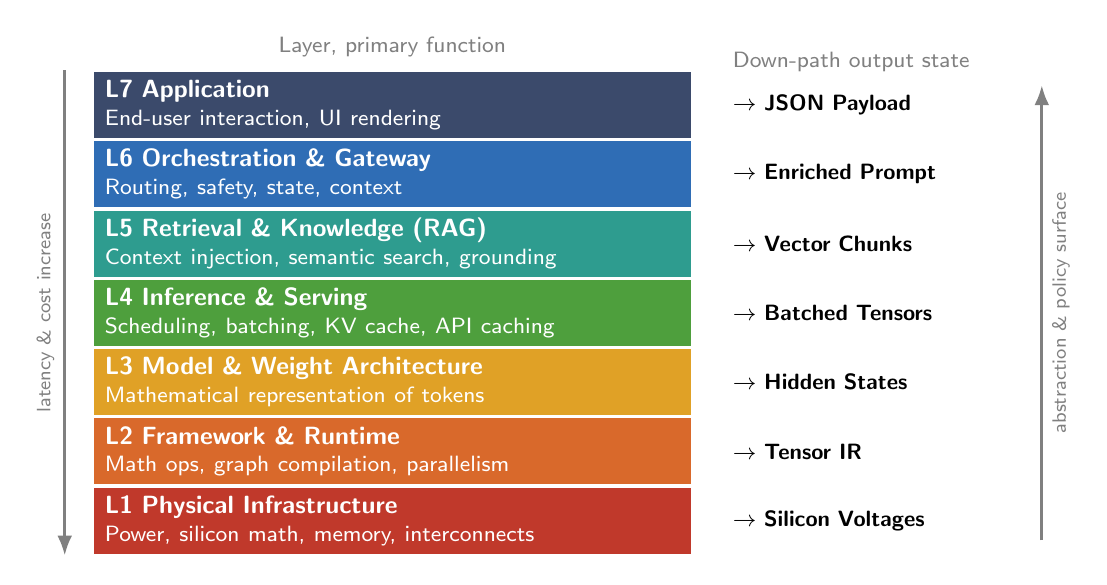
\begin{tikzpicture}[
  lay/.style={draw=white, line width=0.6pt, minimum width=7.6cm, minimum height=0.86cm, text=white, font=\small\sffamily, align=left, text width=7.3cm, inner sep=3pt},
  st/.style={font=\footnotesize\sffamily, align=left, anchor=west, text width=3.7cm}]
\foreach \n/\name/\fun/\col/\state [count=\i] in {
 7/Application/{End-user interaction, UI rendering}/l7/JSON Payload,
 6/Orchestration \& Gateway/{Routing, safety, state, context}/l6/Enriched Prompt,
 5/Retrieval \& Knowledge (RAG)/{Context injection, semantic search, grounding}/l5/Vector Chunks,
 4/Inference \& Serving/{Scheduling, batching, KV cache, API caching}/l4/Batched Tensors,
 3/Model \& Weight Architecture/{Mathematical representation of tokens}/l3/Hidden States,
 2/Framework \& Runtime/{Math ops, graph compilation, parallelism}/l2/Tensor IR,
 1/Physical Infrastructure/{Power, silicon math, memory, interconnects}/l1/Silicon Voltages}{
  \node[lay, fill=\col] (L\n) at (0,-0.88*\i) {\textbf{L\n\ \name}\\[-1pt]{\footnotesize \fun}};
  \node[st] (S\n) at (4.2,-0.88*\i) {$\rightarrow$ \textbf{\state}};
}
\draw[-{Latex[length=2.5mm]}, line width=1pt, gray] ($(L7.north west)+(-0.35,0)$) -- node[left, rotate=90, anchor=south, font=\scriptsize\sffamily, gray]{latency \& cost increase} ($(L1.south west)+(-0.35,0)$);
\draw[-{Latex[length=2.5mm]}, line width=1pt, gray] ($(S1.south east)+(0.1,0)$) -- node[right, rotate=90, anchor=north, font=\scriptsize\sffamily, gray]{abstraction \& policy surface} ($(S7.north east)+(0.1,0)$);
\node[font=\footnotesize\sffamily, gray, anchor=south] at ($(L7.north)+(0,0.05)$) {Layer, primary function};
\node[font=\footnotesize\sffamily, gray, anchor=south west] at ($(S7.north west)+(0,0.05)$) {Down-path output state};
\end{tikzpicture}
\caption{The seven AOSI layers and the data state each layer emits on the down-path (request). The up-path (response) returns logits from L3 to L4 for sampling, and detokenised text through L6 output policy to L7. L5 is normally traversed only on the down-path.}
\label{fig:stack}
\end{figure}

Figure~\ref{fig:stack} shows the stack. We summarise each layer by scope and characteristic failure modes; full component lists, interfaces and metrics are in the technical report~\cite{bhatt2026zenodo}.

\begin{description}[leftmargin=0.6cm, itemsep=3pt, style=unboxed]
\item[L7 Application.] User interaction, request serialisation and rendering of streamed output (chat UIs, IDE assistants, SDKs; SSE or WebSocket streaming). Failure modes: client timeouts shorter than server SLOs, proxies that buffer and defeat streaming, retry storms that amplify load below, rendering stalls misattributed to the model.
\item[L6 Orchestration \& Gateway.] The policy enforcement point: authentication, quotas, model routing, prompt and chat templates, session memory, input and output guardrails, and invocation of L5. Failure modes: prompt bloat from unbounded history, guardrail latency dominating time-to-first-token (TTFT), output moderation that buffers the stream, template mismatch with the model's chat format, prompt injection passing policy checks.
\item[L5 Retrieval \& Knowledge.] Query embedding, approximate-nearest-neighbour search, hybrid retrieval, ACL filtering and reranking over the index \emph{as served}~\cite{lewis2020rag}. Failure modes: retrieval lag (non-resident index, remote hops), low recall from embedding or chunking mismatch, stale indexes, cross-tenant ACL leakage, poisoned documents.
\item[L4 Inference \& Serving.] Tokenisation, admission control, iteration-level scheduling~\cite{yu2022orca}, KV-cache management~\cite{kwon2023paged}, prefix caching, chunked prefill~\cite{agrawal2023sarathi}, disaggregation~\cite{zhong2024distserve}, speculative and constrained decoding. Failure modes: KV-cache exhaustion leading to preemption and time-per-output-token (TPOT) spikes, head-of-line blocking from long prefills, over-batching beyond SLO, low prefix-cache hit rates caused by non-deterministic L6 prefixes.
\item[L3 Model \& Weight Architecture.] The model as mathematics: embeddings, attention variants, MLP or mixture-of-experts blocks, normalisation, output head, and the numerical format of weights, activations and KV cache. Failure modes: numerical instability in low precision, quality regression from quantisation, expert load imbalance, context-length extrapolation failure, configuration mismatch (e.g., positional-encoding scaling).
\item[L2 Framework \& Runtime.] Lowering of the model program to kernels and collective schedules: frameworks, graph compilers, kernel libraries (e.g., IO-aware attention kernels~\cite{dao2022flash}), device runtimes and collective-communication libraries. Failure modes: graph breaks and recompilation jitter, launch-bound execution at small batch, collective stalls from topology-unaware placement, allocator fragmentation.
\item[L1 Physical Infrastructure.] Accelerators, memory hierarchy (HBM, SRAM, host memory), intra- and inter-node interconnects, power and cooling. Failure modes: memory-bandwidth saturation during decode~\cite{yuan2024roofline}, thermal or power throttling, link degradation, hardware errors, noisy neighbours under device partitioning.
\end{description}

\subsection{The data-state chain}
\label{sec:chain}

\begin{figure}[!htbp]
\centering
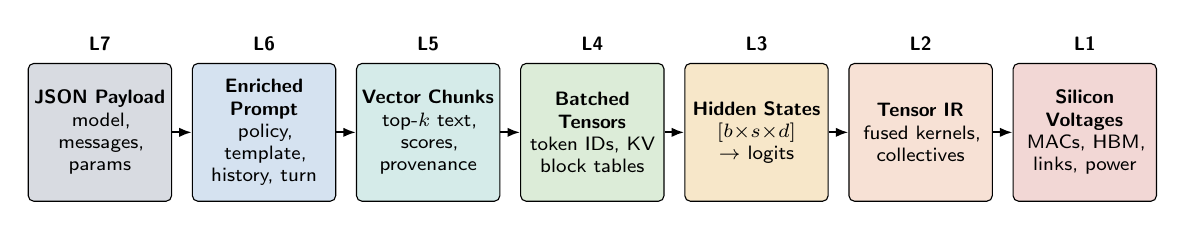
\begin{tikzpicture}[
  box/.style={draw, rounded corners=2pt, font=\scriptsize\sffamily, align=center, minimum height=1.75cm, text width=1.68cm, inner sep=2pt},
  arr/.style={-{Latex[length=1.6mm]}, thick}]
\node[box, fill=l7!20] (a) {\textbf{JSON Payload}\\ model, messages, params};
\node[box, fill=l6!20, right=0.25cm of a] (b) {\textbf{Enriched Prompt}\\ policy, template, history, turn};
\node[box, fill=l5!20, right=0.25cm of b] (c) {\textbf{Vector Chunks}\\ top-$k$ text, scores, provenance};
\node[box, fill=l4!20, right=0.25cm of c] (d) {\textbf{Batched Tensors}\\ token IDs, KV block tables};
\node[box, fill=l3!25, right=0.25cm of d] (e) {\textbf{Hidden States}\\ $[b{\times}s{\times}d]$ $\rightarrow$ logits};
\node[box, fill=l2!20, right=0.25cm of e] (f) {\textbf{Tensor IR}\\ fused kernels, collectives};
\node[box, fill=l1!20, right=0.25cm of f] (g) {\textbf{Silicon Voltages}\\ MACs, HBM, links, power};
\foreach \x/\y in {a/b,b/c,c/d,d/e,e/f,f/g} \draw[arr] (\x) -- (\y);
\foreach \n/\l in {a/L7,b/L6,c/L5,d/L4,e/L3,f/L2,g/L1} \node[font=\scriptsize\sffamily\bfseries, above=1pt of \n] {\l};
\end{tikzpicture}
\caption{The canonical down-path data-state chain. Each state is the representation of a request as it leaves a layer and is the natural capture point for boundary telemetry.}
\label{fig:chain}
\end{figure}

Principle P2 requires a named data state at every boundary (Figure~\ref{fig:chain}). On the down-path: L7 emits a \textbf{JSON payload} (e.g., model, messages, tools, sampling parameters, stream flag); L6 emits an \textbf{enriched prompt}---an ordered sequence of system policy, template, session state, grounding slot and user turn, with routing decision and policy verdicts attached; L5 returns \textbf{vector chunks}---ranked retrieved passages with scores and provenance, merged by L6 into the prompt; L4 forms \textbf{batched tensors}---token and position IDs, attention metadata, KV-cache block tables and batch-slot assignments; L3 produces \textbf{hidden states}---per-block activations and, finally, logits; L2 lowers the computation to \textbf{tensor IR}---captured or compiled graphs, fused kernels and collective schedules; and L1 executes it as \textbf{silicon voltages}---the physical switching behind multiply--accumulate operations, memory transactions and link signalling, observable as utilisation, bandwidth and power. The last label is deliberately physical shorthand: what is observable at L1 is switching activity expressed as hardware counters, memory and link throughput, power and temperature, not voltages as such.

Two properties make the chain useful rather than decorative. First, each state has a measurable size that propagates downward: enriched-prompt token count at L6/L4 determines prefill work at L3--L1; $k$ and chunk length at L5/L6 determine part of that token count; batch composition at L4/L3 determines the arithmetic intensity seen at L1. Second, each state is a \emph{checkpoint for blame}: if the state entering a layer is unchanged and the layer's span grew, the layer itself is implicated; if the incoming state changed, the layer above is implicated (Section~\ref{sec:triage}).

\paragraph{Request lifecycle.} On the down-path, L6 authenticates, routes, applies guardrails and templates, calls L5, and hands the enriched prompt to L4, which tokenises, checks the prefix cache, allocates KV blocks and admits the sequence into a batch; L3--L1 execute the prefill forward pass. The first sampled token fixes TTFT. Each subsequent token is a decode iteration that reads weights and the KV cache from device memory; at typical batch sizes decode tends to be memory-bandwidth-bound~\cite{yuan2024roofline}, so TPOT is governed largely by L4 batching and KV behaviour and by L1 memory bandwidth. Tokens are detokenised at L4 and stream through L6 output policy to L7.

\section{Cross-Layer Diagnostics}
\label{sec:diag}

\subsection{Principle}
A protocol analyser makes network faults tractable by decoding a captured unit layer by layer. AOSI proposes the analogous discipline for generative AI: \emph{each request should produce a trace in which every span is attributed to exactly one AOSI layer, and each boundary hand-off is timestamped}. Concretely, an AOSI-aligned deployment propagates one trace context from L7 through L4~\cite{w3ctracecontext,sigelman2010dapper}; tags each span with a layer attribute alongside OpenTelemetry generative AI attributes~\cite{otelgenai}; exports serving-engine and device metrics on a common time base with node, device and replica labels so that spans can be joined to device telemetry; and captures framework-level profiles on demand.

\subsection{Latency decomposition}
For a streamed response with $N_{\text{out}}$ output tokens,
\begin{align}
E2E &\approx \text{TTFT} + (N_{\text{out}}-1)\cdot\text{TPOT},\\
\text{TTFT} &\approx t_{L7} + t_{L6}^{\text{gw}} + t_{L6}^{\text{guard,in}} + t_{L5} + t_{L4}^{\text{queue}} + t_{L4}^{\text{tok}} + t_{\text{prefill}}^{L3\text{--}L1} + t_{\text{up}},\\
\text{TPOT} &\approx t_{L4}^{\text{sched}} + t_{\text{decode}}^{L3\text{--}L1} + t_{L6}^{\text{guard,out}}.
\end{align}
The decomposition halves the search space. TTFT inflated with TPOT normal points \emph{above} L4 compute (L6 overhead, L5 retrieval, L4 queueing, or longer prompts). TPOT inflated with TTFT normal points at or \emph{below} L4 decode (KV pressure, batch growth, memory bandwidth, throttling, collectives) or at buffering output guardrails in L6. Both inflated suggests systemic causes: overload, device degradation, or retry storms.

\subsection{Discriminating three commonly confused causes}
Table~\ref{tab:discrim} lists signals that separate L5 retrieval lag, L4 KV-cache pressure and L1 memory-bandwidth saturation, each of which can surface as ``the model is slow''. The signatures follow from the mechanisms described in the serving and roofline literature~\cite{kwon2023paged,yuan2024roofline}; they are hypotheses to be calibrated per deployment, not measured thresholds.

\begin{table}[!htbp]
\centering
\caption{Discriminating signals for three causes of perceived slowness. Signatures are derived from mechanism, not measurement, and must be calibrated per deployment.}
\label{tab:discrim}
\small
\begin{tabularx}{\textwidth}{@{}>{\raggedright\arraybackslash}p{2.1cm}YYY@{}}
\toprule
& \textbf{L5 retrieval lag} & \textbf{L4 KV-cache pressure} & \textbf{L1 memory-bandwidth saturation}\\
\midrule
Latency signature & TTFT up; TPOT unchanged & TPOT up and spiky; TTFT up if admission blocks & TPOT up smoothly with batch and context\\
Trace location & L5 span grows before any L4 span & L4 queue span grows; decode shows preemption gaps & L4 decode span grows uniformly per step\\
Engine / device signals & Engine and device normal & KV utilisation near capacity; preemption counters rise & Memory-bandwidth utilisation pinned near ceiling; compute pipes comparatively idle\\
Isolation test & Replay with retrieval bypassed and an equal-length fixed context & Replay with reduced concurrency or larger KV budget & Fixed-batch sweep of context length or batch size\\
Remediate at & Index residency, co-location, smaller $k$ & Prefix caching, KV quantisation, admission limits, chunked prefill & Weight/KV quantisation, speculative decoding, scale-out\\
\bottomrule
\end{tabularx}
\end{table}

\subsection{Triage procedure}
\label{sec:triage}
Diagnosis proceeds top-down for attribution and bottom-up for confirmation: (1)~quantify the symptom (TTFT, TPOT, E2E, error rate, goodput or quality; percentile and window); (2)~decompose it into TTFT and TPOT movement; (3)~walk the trace top-down (L7$\rightarrow$L4) against a baseline---the first layer whose span distribution shifted is the \emph{candidate layer}; (4)~check the boundary state entering that layer (e.g., prompt tokens at L6/L4, $k$ at L5/L6, batch size at L4/L3), since a changed input implicates the layer above; (5)~correlate with lower-layer telemetry (engine metrics, framework profiles, device counters); (6)~run the candidate layer's isolation test, changing exactly one variable; (7)~confirm bottom-up that lower layers are healthy under the test; (8)~remediate at the owning layer and re-measure the original symptom; and (9)~record the incident with its AOSI layer attribution.
Step~9 is what would make AOSI testable at scale: a corpus of layer-attributed incidents is the dataset our evaluation plan requires (Section~\ref{sec:eval}).

\section{Security Mapping}
\label{sec:security}

Under principle P7, each threat is placed at the layer where it materialises. Table~\ref{tab:owasp} maps the OWASP Top 10 for LLM Applications (2025)~\cite{owasp2025llm} onto AOSI. The mapping is the author's; it is intended to be contested and refined. Two observations follow. First, several risks are multi-layer by nature: prompt injection is \emph{enforced against} at L6 but \emph{arrives} via L7 (direct) or L5 (indirect, through retrieved content~\cite{greshake2023indirect}); misinformation is the joint outcome of grounding (L5), model behaviour (L3) and presentation (L7). Second, a layer index exposes control gaps that a flat list hides: an architecture whose only control for LLM04 and LLM08 is an L6 guardrail has no control at the layer (L5 or L3) where poisoning materialises. The same index can be applied to MITRE ATLAS techniques~\cite{mitreatlas} and the NIST adversarial ML taxonomy~\cite{nist2025aml}; we leave that mapping to future work.

\begin{table}[!htbp]
\centering
\caption{OWASP Top 10 for LLM Applications (2025) mapped to the AOSI layer(s) where each risk materialises, with representative layer-local controls. Author's mapping; illustrative, not normative.}
\label{tab:owasp}
\small
\begin{tabularx}{\textwidth}{@{}>{\raggedright\arraybackslash}p{4.1cm}>{\raggedright\arraybackslash}p{2.6cm}Y@{}}
\toprule
\textbf{OWASP risk (2025)} & \textbf{Primary layer(s)} & \textbf{Representative controls at that layer}\\
\midrule
LLM01 Prompt Injection & L6 (arrives via L7 or L5) & Separation of system, user and retrieved content; input classifiers; least-privilege tool scopes; L5 content scanning\\
LLM02 Sensitive Information Disclosure & L6, L5, L3 & Output filtering and redaction (L6); ACL-filtered retrieval (L5); training-data extraction testing (L3)\\
LLM03 Supply Chain & L2, L3 & Pinned, verified dependencies and SBOMs (L2); signed, hash-verified model artefacts and provenance (L3)\\
LLM04 Data and Model Poisoning & L3 (weights), L5 (corpus) & Model provenance and red-teaming (L3); ingestion integrity and provenance checks (L5)\\
LLM05 Improper Output Handling & L6, L7 & Schema validation (L6); rendering that never executes untrusted content (L7)\\
LLM06 Excessive Agency & L6 (future L8) & Tool permission scoping, human approval gates, action budgets\\
LLM07 System Prompt Leakage & L6 & Secrets kept out of prompts; leakage detection on output\\
LLM08 Vector and Embedding Weaknesses & L5 & Vector-store access control; tenant isolation; encryption at rest\\
LLM09 Misinformation & L5, L3, L7 (cross-layer) & Grounding evaluation and freshness (L5); quality evaluation (L3); citation display (L7)\\
LLM10 Unbounded Consumption & L4, L6 & Token and time budgets (L4); rate limits and quotas (L6)\\
\bottomrule
\end{tabularx}
\end{table}

Beyond OWASP, AOSI surfaces threats that application-level lists tend not to emphasise: cross-request leakage through shared prefix or KV caches (L4), unsafe deserialisation of model files and compromised kernels or compilers (L2), and hardware side channels or memory residue between tenants (L1). An AOSI-aligned description of a system should state, per layer, which threats are in scope and which controls apply, and should not rely on a single layer as the sole control for threats that materialise at another.

\section{Illustrative Worked Example}
\label{sec:case}

\noindent\fbox{\parbox{\dimexpr\linewidth-2\fboxsep-2\fboxrule}{\small\textbf{Note.} This section is a constructed, hypothetical walk-through intended only to show how the model's vocabulary and procedure are applied. It does not describe a real incident and reports no measurements.}}

\medskip
\noindent\textbf{Setting.} Consider an internal question-answering assistant: a web client (L7) calls an AI gateway that applies a system prompt, conversation history and guardrails (L6); the gateway retrieves policy documents from a vector index (L5); a self-hosted serving engine with continuous batching and paged KV cache (L4) runs a quantised transformer (L3) compiled with a standard framework (L2) on a multi-GPU node (L1).

\paragraph{Symptom A: ``the assistant got slow this week''.} Step~1 restates the complaint as a metric: suppose the operators observe that p95 TTFT has risen relative to the previous week while TPOT has not. Step~2 therefore directs attention above L4 compute. Walking the trace (Step~3), they compare per-layer span distributions; suppose the L5 span is unchanged but the L4 queue and prefill spans have grown. Step~4 checks the boundary state at L6/L4 and finds that enriched-prompt token counts have grown, because a recent L6 change now replays full conversation history instead of a summary. The input to L4 changed, so the layer \emph{above} is implicated: the root cause is at L6, even though the time is spent at L4--L1. The isolation test (Step~6) replays the same requests with history truncated; if TTFT returns to baseline, the attribution is confirmed. The remediation is at L6 (history windowing or summarisation), not at L4 (adding replicas), which would only have masked the cause. The incident is recorded as \emph{L6, prompt growth, manifesting at L4}.

\paragraph{Symptom B: ``the assistant cites the wrong policy''.} Latency is normal, so the decomposition is uninformative and the operators move to quality signals. The AOSI boundary states structure the questions: were the \emph{vector chunks} returned at L5/L6 the right documents (a retrieval-evaluation question at L5)? Did they reach the \emph{enriched prompt} intact and in the intended position (an L6 template question)? Given correct context, did the model use it (an L3 question, testable by replaying the identical enriched prompt against a reference-precision model)? Each question isolates one layer by holding the incoming state fixed. If, say, the index had not been refreshed after a policy update, the fault is an L5 freshness failure, which also corresponds to OWASP LLM09 and is mitigated at L5 rather than by a stricter L6 output filter.

\paragraph{What the example shows and does not show.} The example demonstrates that the vocabulary distinguishes \emph{where time is spent} from \emph{where the cause lies}, and that boundary states give a principled order of questions. It does not show that practitioners using AOSI diagnose faster or more accurately than without it; that is the hypothesis our evaluation plan tests.

\section{Discussion, Limitations and Evaluation Plan}
\label{sec:discussion}

\subsection{Limitations and threats to validity}
\begin{itemize}[leftmargin=*,itemsep=2pt]
\item \textbf{No empirical validation.} The layer boundaries, discriminating signals and security mapping are argued from mechanism and the literature, not measured. Thresholds in the technical report are explicitly illustrative.
\item \textbf{No standards adoption.} AOSI is a single-author proposal. It has not been reviewed or adopted by ISO/IEC, ITU-T, IETF, NIST or any other body.
\item \textbf{Construct validity of boundaries.} Real systems violate strict layering: serving engines ship their own kernels (L4/L2), gateways cache responses (L6 behaving like L4), and embedding models are served by L4 engines inside L5. AOSI handles these through principle P1 (describe a component once per layer it occupies) and P3 (document couplings), but whether this remains workable for real inventories is untested.
\item \textbf{Ordering of L5.} Retrieval is placed between orchestration and serving because it transforms the prompt before serving; it is, however, invoked by L6 and is not on the up-path. Alternative placements (e.g., retrieval as a peer service of L6) are defensible.
\item \textbf{Scope.} Training, fine-tuning and data pipelines are excluded; agentic, multi-step and multi-agent workflows are reserved for future layers. Many current production issues arise exactly there.
\item \textbf{Author bias.} The comparison in Table~\ref{tab:compare} and the mapping in Table~\ref{tab:owasp} were produced by the model's author. Independent replication of both is needed.
\item \textbf{Rapid technological change.} Named components will date quickly. The model's claim is that the \emph{layers and boundary states} are stable even as occupants change; this is itself a hypothesis.
\end{itemize}

\subsection{Evaluation plan}
\label{sec:eval}
We propose three studies, ordered by cost.
\begin{enumerate}[leftmargin=*,itemsep=2pt]
\item \textbf{Incident classification study.} Collect publicly available post-incident reports and issue-tracker reports from open-source serving engines, gateways and RAG frameworks. Two or more independent raters classify each by AOSI layer of \emph{root cause} and of \emph{manifestation}, using a written codebook. Outcomes: inter-rater agreement (e.g., Cohen's or Fleiss' $\kappa$), the fraction of reports that cannot be assigned to a layer (a direct test of coverage), and the frequency with which root cause and manifestation layers differ (a test of the claim that the distinction matters).
\item \textbf{Practitioner survey and card-sorting.} Ask practitioners across application, platform, ML and infrastructure roles to sort component and symptom cards into layers, and to rate the clarity and usefulness of each boundary. Outcomes: agreement with AOSI's assignments, boundaries with systematic disagreement, and candidate revisions.
\item \textbf{Controlled diagnosis experiment.} Inject single, known faults (e.g., retrieval delay, KV-budget reduction, prompt growth, power capping) into an instrumented open-source stack, and compare time-to-correct-attribution and accuracy for participants with and without AOSI-tagged traces. This is the only study that would test the model's central practical claim.
\end{enumerate}
Results from any of these studies, including negative results, would warrant revision of the model.

\subsection{Future layers}
Three extensions are reserved and informative: an L8 for agentic workflows (planning, tool use, multi-agent coordination), where ACE~\cite{shapiro2023ace}, Lu et al.'s agent architecture~\cite{lu2024agents} and Rodrigo-Gin\'es's interoperability stack~\cite{rodrigogines2025osi} are natural points of alignment; an L9 or cross-cutting plane for distributed and federated inference across sites; and a global optimisation plane relating per-layer controls to end-to-end goals such as energy per output token. An open question is whether these are layers at all, or planes that cut across L1--L7.

\section{Conclusion}
\label{sec:conclusion}
Generative AI inference spans tiers that are engineered, observed and secured separately, and the field lacks a shared way to say where a problem lives. AOSI borrows OSI's method---ordered layers, stable boundaries and named data units---and applies it to the execution path of a single generative request, from silicon to application. Its specific contribution is the combination of full-depth layering, a named data state at every boundary, a layer-isolation diagnostic method built on those states, and a layer-indexed security mapping; it does not claim to be the first layered or OSI-inspired model for AI. The model is unvalidated, and its value depends on whether practitioners can apply it consistently and whether it shortens diagnosis. We have outlined studies to test both, and we invite counter-examples and alternative boundaries.

\section*{Availability}
The full specification (version 1.2.1), including per-layer interfaces, metrics, failure modes, a diagnostic matrix and proposed telemetry attributes, is archived at \url{https://doi.org/10.5281/zenodo.24073122}~\cite{bhatt2026zenodo} and maintained at \url{https://github.com/CodingThrill0012/aosi-model} under CC-BY-4.0.

{\footnotesize\setlength{\bibsep}{1pt}
\bibliographystyle{unsrtnat}
\bibliography{refs}}

\end{document}
